\section{Introduction to the FWI}
\subsection{Seismic Acquisition}


% ============================================
% ====== Frame : Pb inverse  ================= 1
% ============================================
\begin{frame}{Seismic Imaging}


  \begin{figure}
    \def\svgwidth{1.0\linewidth}
    \input{images/intro_1.pdf_tex}
  \end{figure}

\end{frame}

\begin{frame}[noframenumbering]{Seismic Imaging}


  \begin{figure}
    \def\svgwidth{1.0\linewidth}
    \input{images/intro_2.pdf_tex}
  \end{figure}

\end{frame}

\newcommand\hideit[1]{%
  \only<0| handout:1>{\mbox{}}%
  \invisible<0| handout:1>{#1}}



% ============================================
% ====== Frame : FWI Workflow 1       ======== 2
% ============================================
\subsection{FWI Workflow}

\begin{frame}{Seismic Imaging}
\small
\vspace{-3.67cm}
\begin{columns}
\column{\dimexpr\paperwidth-10pt}
\begin{figure}
\def\svgwidth{1.0\linewidth}
\input{images/data.pdf_tex}
\end{figure}
\end{columns}
\end{frame}

\begin{frame}[noframenumbering]{FWI Workflow}
  \vspace{-0.5cm}
  \begin{columns}
    \column{\dimexpr\paperwidth-10pt}
    \begin{figure}
      \def\svgwidth{1.0\linewidth}
      \input{images/data_2.pdf_tex}
    \end{figure}
  \end{columns}
  \uncover<2->{
    \begin{equation}
      \CF(\model) = \frac{1}{2}||\textcolor{blue}{d_{obs}}-\textcolor{red}{\mathcal{F}(\model)}||^2
    \end{equation}
    \vspace{-0.2cm}
 \begin{itemize}
   \item $\mathcal{F}(m)$ is the restriction on the receivers of the simulated waves in the medium $\model$. (With $\model = \velocity, \density, \bulkmodulus$...)
   \item FWI: minimization problem by using adjoint state method \footcite{tarantolaInversionSeismicReflection1984} \footcite{laillySequenceStackMigrations1983}
 \end{itemize}

  }
\end{frame}



% ============================================
% ====== Frame : FWI Workflow 2       ======== 3
% ============================================


\begin{frame}{FWI Workflow}
\begin{figure}
  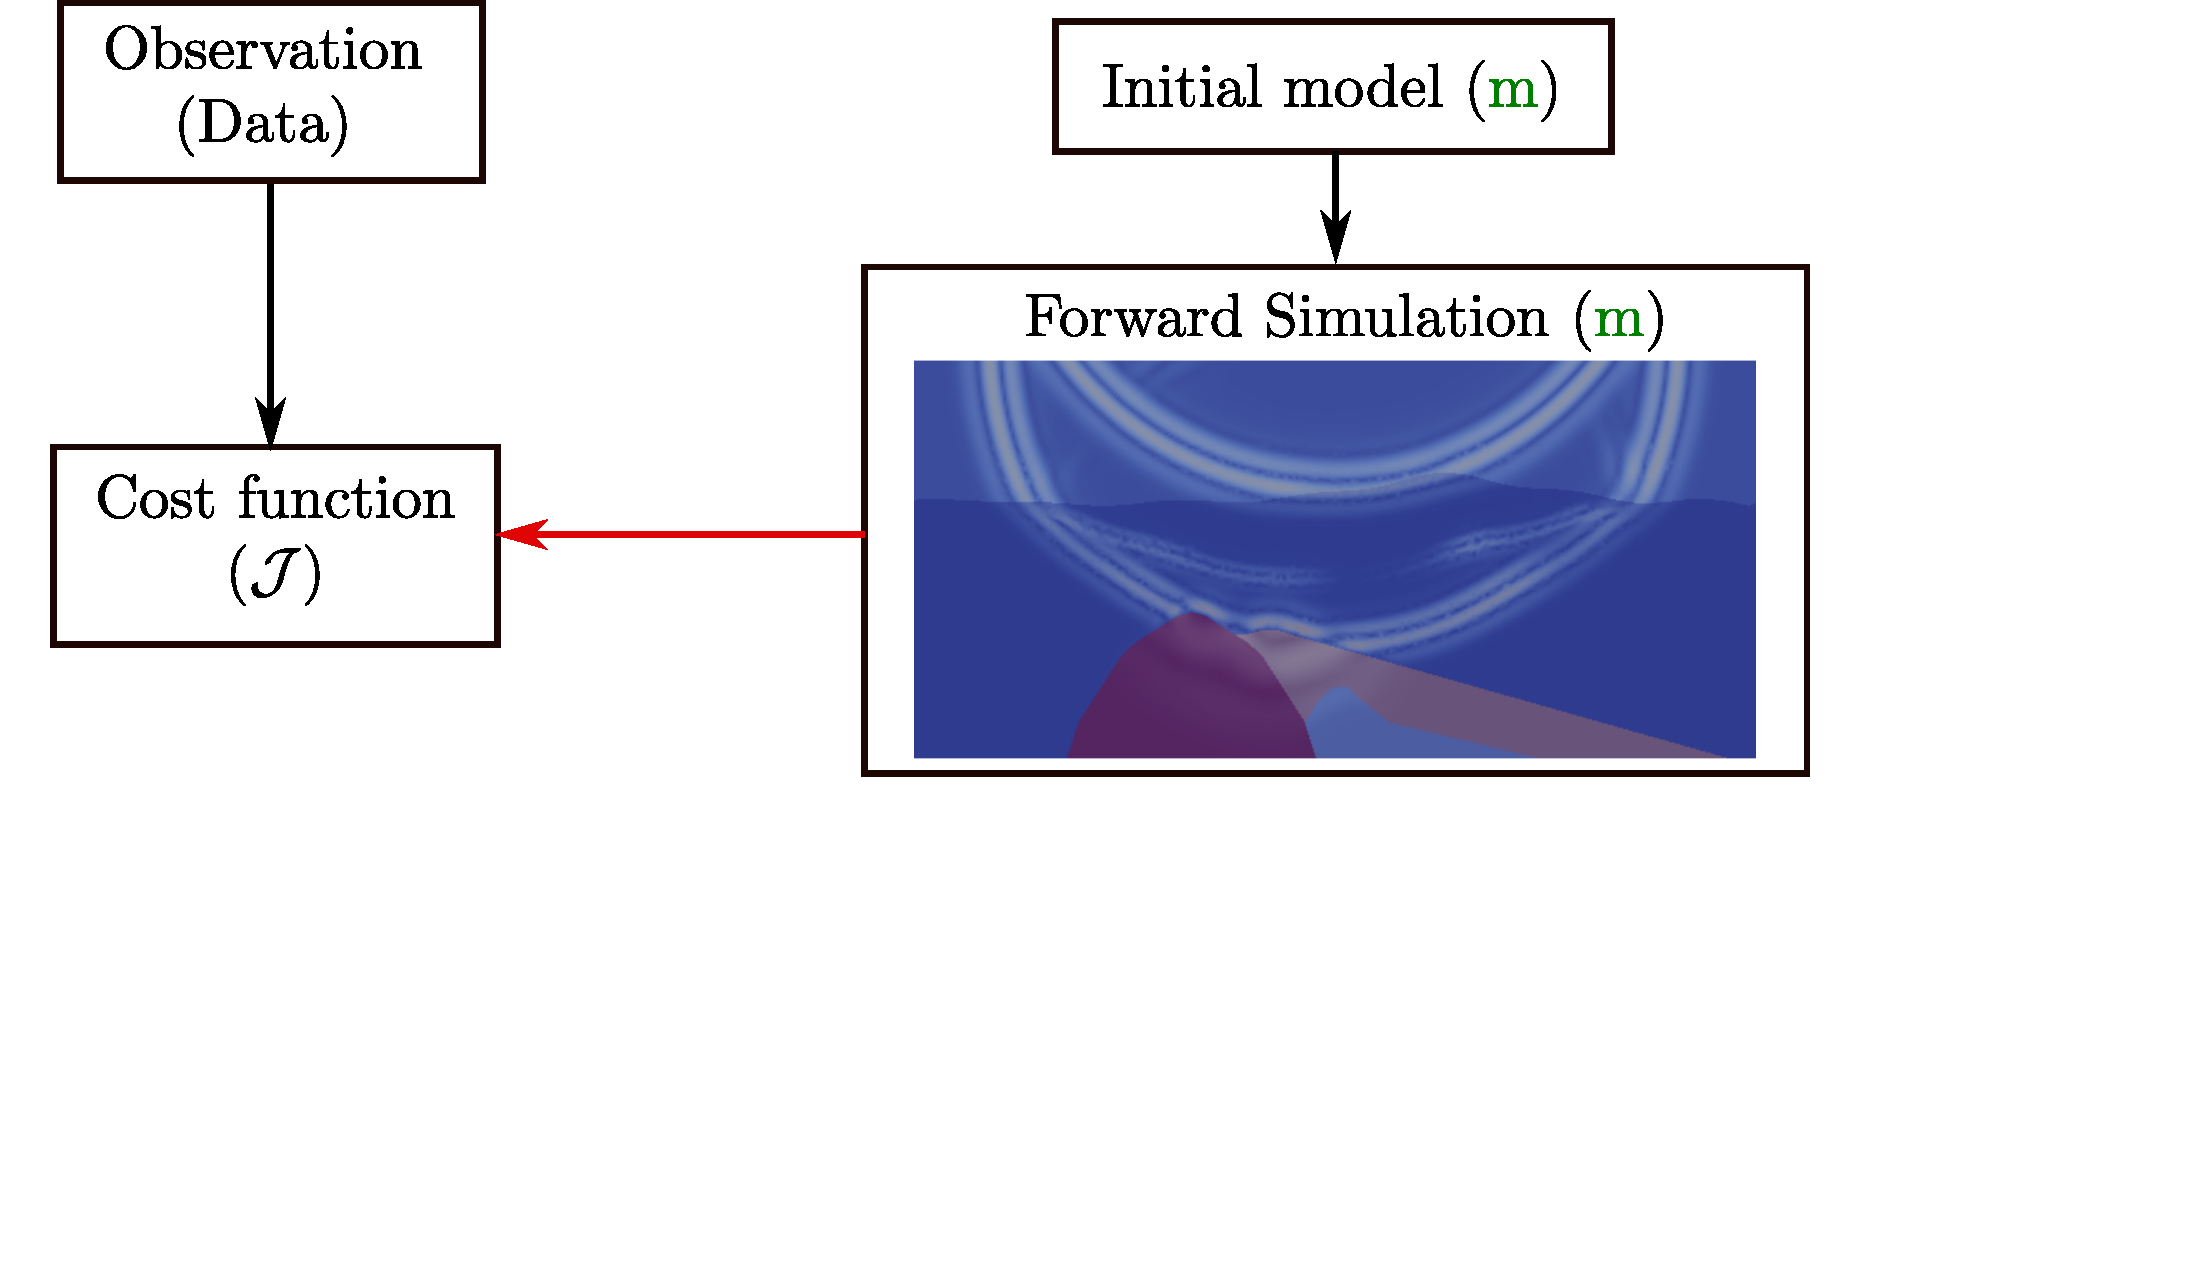
\includegraphics[scale=0.31]{image/fwi_workflow_grad2.pdf}
\end{figure}
\end{frame}

\begin{frame}[noframenumbering]{FWI Workflow}
\begin{figure}
  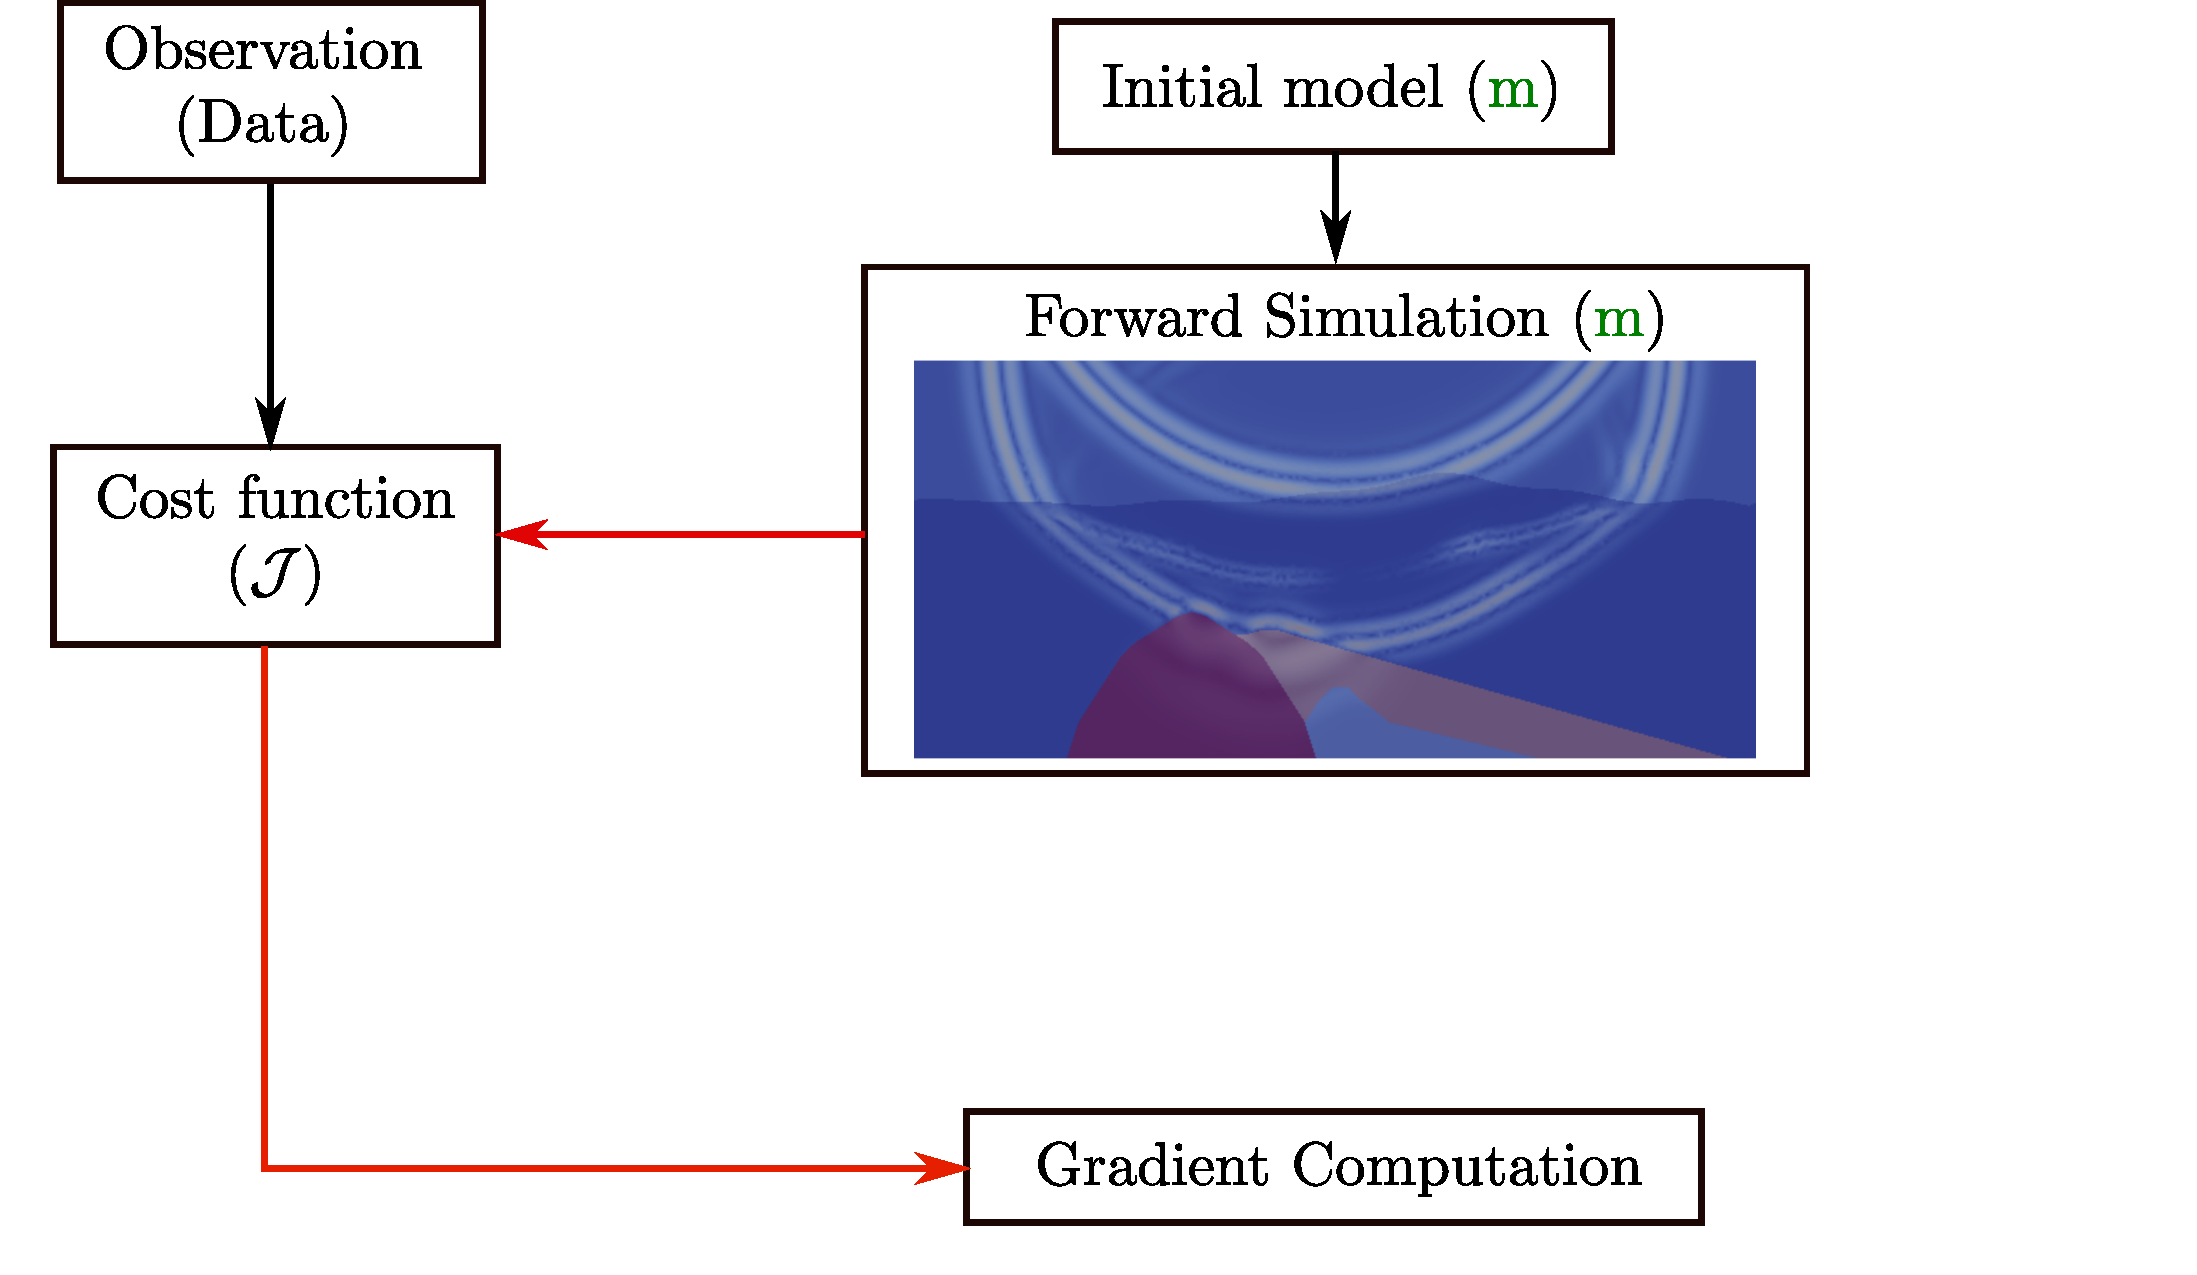
\includegraphics[scale=0.31]{image/fwi_workflow_grad1.pdf}
\end{figure}
\end{frame}

\begin{frame}[noframenumbering]{FWI Workflow}
\begin{figure}
  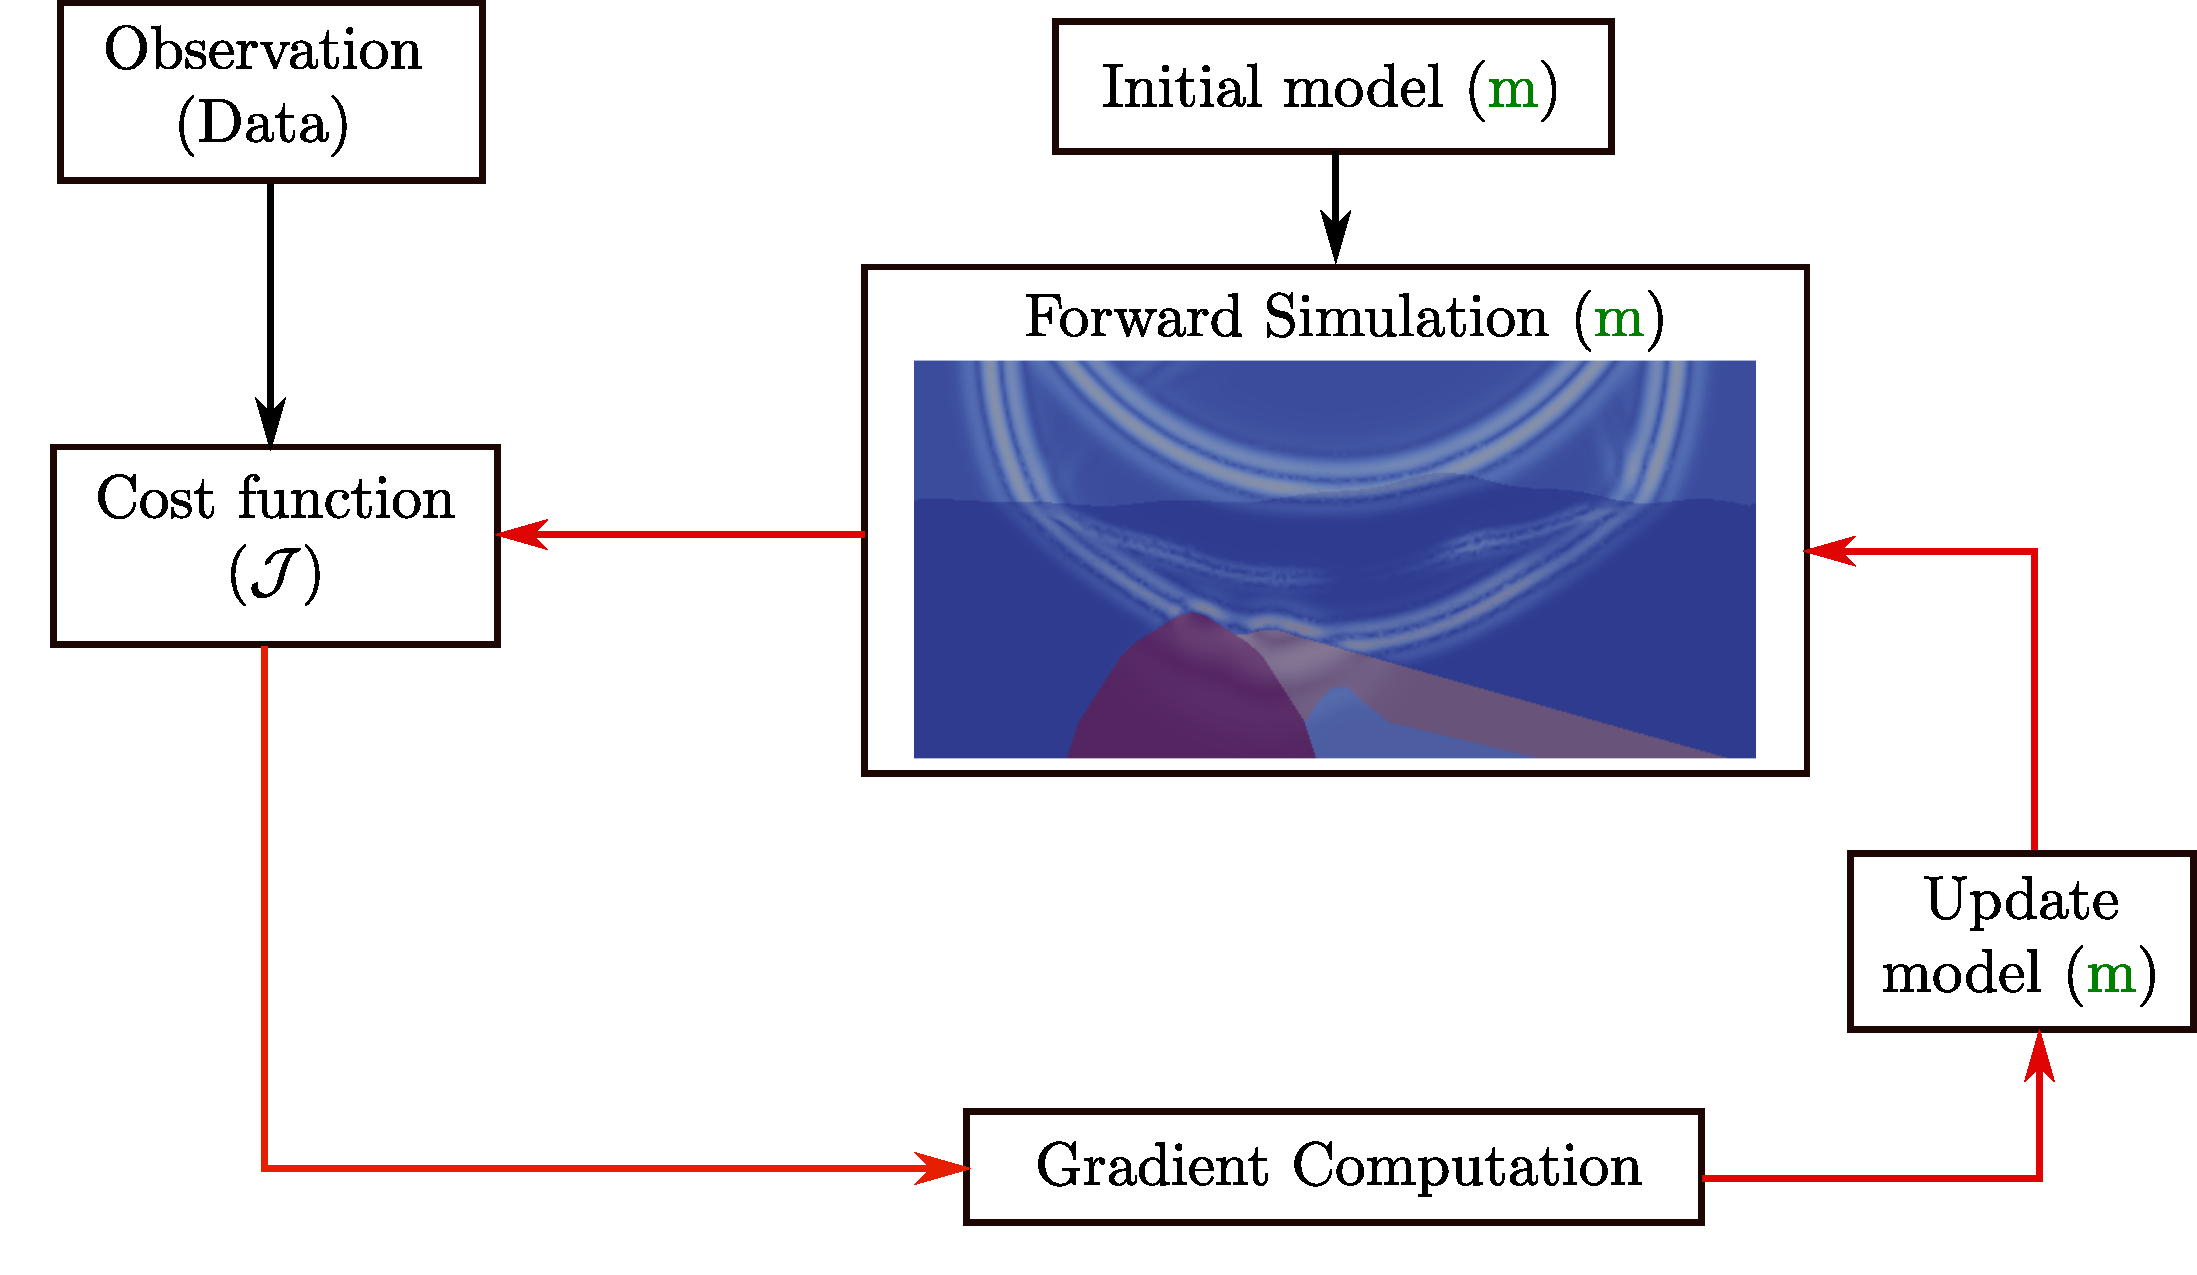
\includegraphics[scale=0.31]{image/fwi_workflow_grad.pdf}
\end{figure}
\end{frame}

\begin{frame}[noframenumbering]{FWI Workflow}
\begin{figure}
  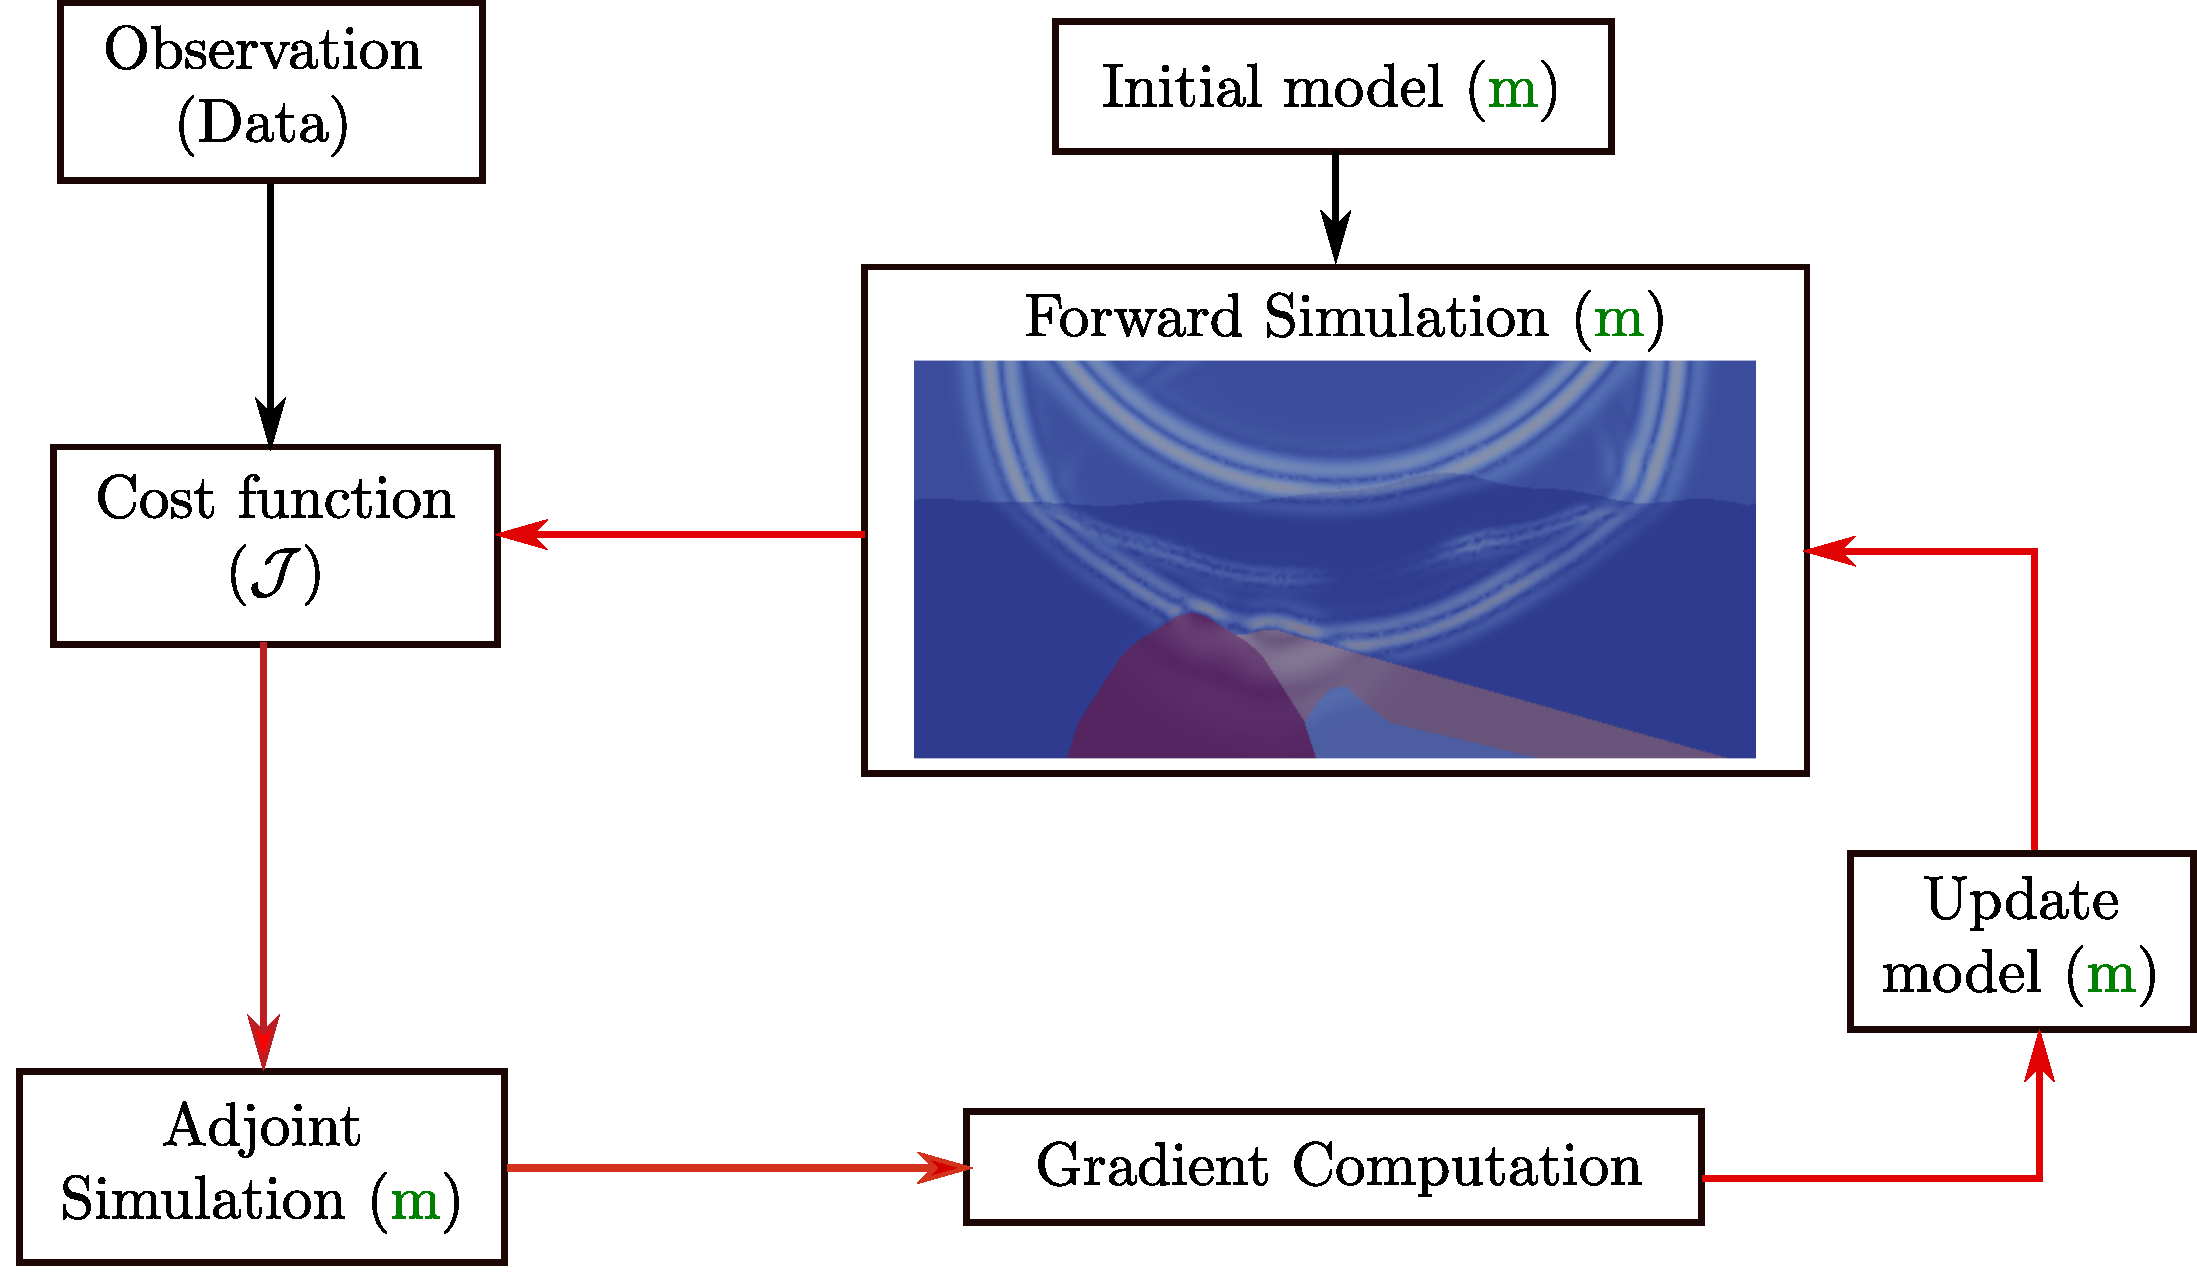
\includegraphics[scale=0.31]{image/fwi_workflow.pdf}
\end{figure}
\end{frame}

\begin{frame}[noframenumbering]{FWI Workflow}
\begin{figure}
  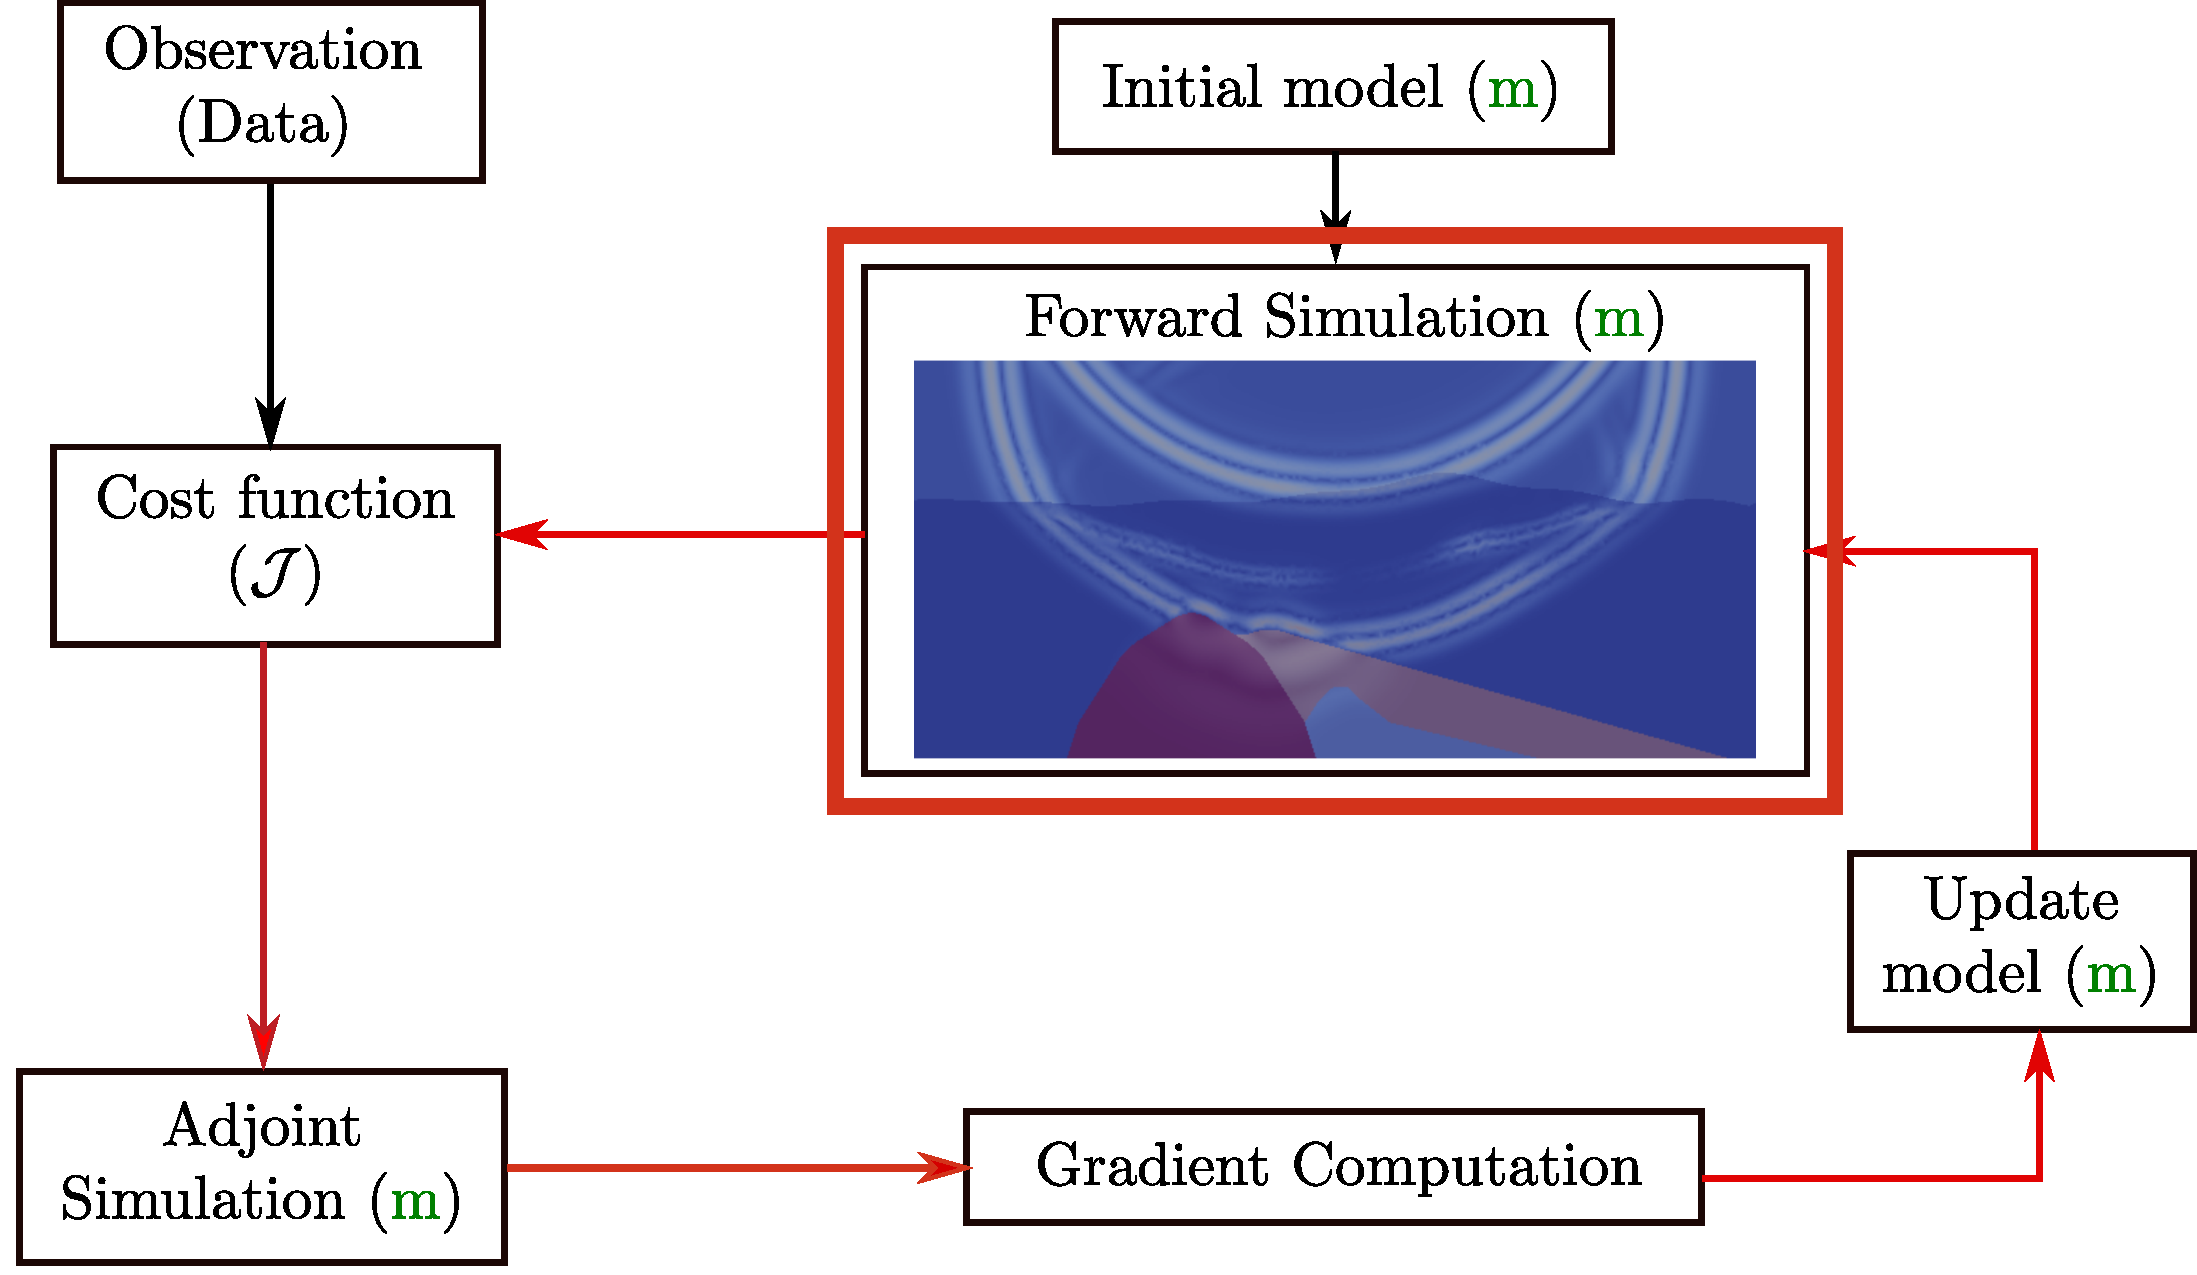
\includegraphics[scale=0.31]{image/fwi_workflow_red.pdf}
\end{figure}
\end{frame}
